\documentclass[a4paper]{article}

\usepackage{amsmath}
\usepackage{amssymb,amsfonts}
\usepackage[catalan]{babel} % Language 
\usepackage{fontspec} 
\usepackage[margin=2cm]{geometry}
\usepackage{graphicx}
\usepackage{float}
\usepackage{xcolor}
\usepackage{listings}

\usepackage{xparse}
\setlength{\parindent}{0pt}
\setlength{\parskip}{0.2cm}

\usepackage{color}
\lstset{ %
	language=R,                     % the language of the code
	basicstyle=\footnotesize,       % the size of the fonts that are used for the code
	%numbers=left,                   % where to put the line-numbers
	%numberstyle=\tiny\color{gray},  % the style that is used for the line-numbers
	stepnumber=1,                   % the step between two line-numbers. If it's 1, each line
	% will be numbered
	numbersep=5pt,                  % how far the line-numbers are from the code
	backgroundcolor=\color{white},  % choose the background color. You must add \usepackage{color}
	showspaces=false,               % show spaces adding particular underscores
	showstringspaces=false,         % underline spaces within strings
	showtabs=false,                 % show tabs within strings adding particular underscores
	%frame=single,                   % adds a frame around the code
	%rulecolor=\color{black},        % if not set, the frame-color may be changed on line-breaks within not-black text (e.g. commens (green here))
	tabsize=2,                      % sets default tabsize to 2 spaces
	captionpos=b,                   % sets the caption-position to bottom
	breaklines=true,                % sets automatic line breaking
	breakatwhitespace=false,        % sets if automatic breaks should only happen at whitespace
	title=\lstname,                 % show the filename of files included with \lstinputlisting;
	% also try caption instead of title
	keywordstyle=\color{blue},      % keyword style
	commentstyle=\color{dkgreen},   % comment style
	stringstyle=\color{mauve},      % string literal style
	escapeinside={\%*}{*)},         % if you want to add a comment within your code
	morekeywords={*,...},
	          % if you want to add more keywords to the set
	alsoletter={.}        % if you want to add more keywords to the set
} 

\graphicspath{{images/}}
\DeclareMathOperator{\diag}{diag}

\title{Problemes APA \\ Problema 11: Pràctica amb la xarxa MLP}
\author{Lluc Bové}
\date{Q1 2016-17}

\begin{document}

\maketitle

Es disposa de 48 mesures de roques d'un dipòsit de petroli. L'objectiu és modelar la permeabilitat en funció de l'àrea, el perímetre i la forma. En primer lloc transformem les dades per ajudar a l'ajust del model:

\begin{lstlisting}
	library(datasets)
	data(rock)
	?rock
	
	rock.x <- data.frame(area = scale(rock$area), peri = scale(rock$peri),shape = scale(rock$shape))
	rock.y <- log(rock$perm)
\end{lstlisting}

Entreneu una xarxa \textit{MLP} per aprendre la tasca. Donat el baix número d'exemples, useu \textit{leave-one-out cross-validation} i regularització per trobar la millor xarxa. Per avaluar el model, feu una gràfica de resposta predita vs. observbada i guieu-vos per l'error quadràtic normalitzat (normalized root MSE) del laboratori 3.

Primer hem de decidir quantes dades seràn de test i quantes de training. Decidim usar un 75\% de les dades per training i la resta per test. Per a selaccionar una mostra aleatòria fem servir la funció \lstinline|sample|. També definim la funció \lstinline|norm.mse| que és l'error quadràtic normalitzat que es defineix com a: $$\frac{\sum_{i = 0}^{N}t_i - y(x_i)}{(N - 1) Var(t)}$$ 

on $t$ són les mostres de la variable que volem predir, $x$ la resta de variables, $N$ la mida de les dades, $y$ el model en qüestio i $Var$ és la variança mostral.

Primer creem una xarxa neuronal sense regularització i amb 4 neurones a la capa oculta. Veiem que obtenim valors del 15\% per l'error de training i 61\% pel de test. Probablament estiguem sobreajustant. Així doncs apliquem regularització, provem per valors de $\lambda$ de $10^{-5}$ fins a 0, en increments de $0.1$. Ho fem aplicant \textit{LOOCV}. Trobem que la millor $\lambda$ és de $0.063$ i calculem l'error amb un model que la utilitzi. Trobem un error de 9\% i 17\% per els errors de training i test respectivament. Veiem com hem aconseguit reduir l'error de test. Finalment representem el valor de permeabilitat observat respecte el que predim amb el model, i obtenim el següent gràfic:

\begin{figure}[H]
	\centering
	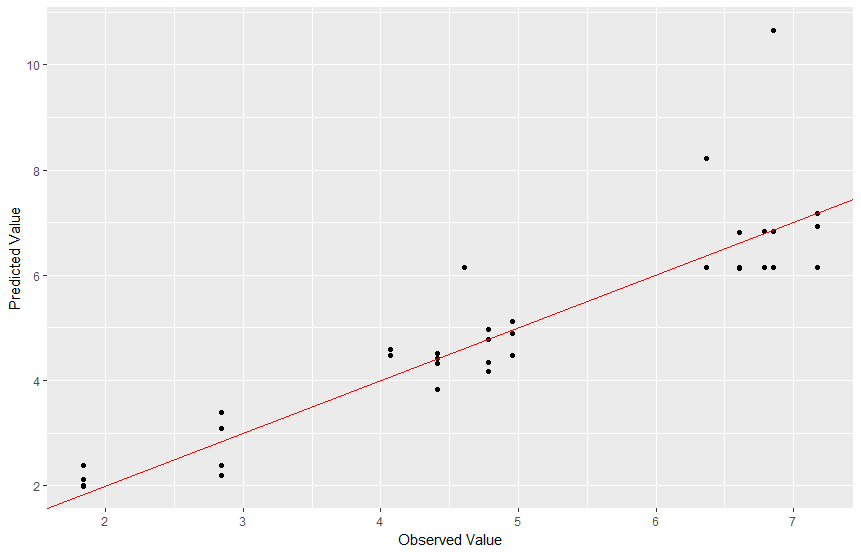
\includegraphics[scale=0.45]{plot}
\end{figure}

La línia vermella representa la recta on haurien d'estar situats els punts si la predicció fos perfecta. En tot cas veiem que alguns punts no es desvien gaire i tenen poca variabilitat però alguns punts la predicció no és acurada. El model és limitat per el baix nombre de dades.




\end{document}